\documentclass[11pt,tikz]{standalone}
\usepackage[OT1]{eulervm}
\usepackage{libertine}

\usepackage{xcolor}

% ------- %
% Colours %
% ------- %

% Playroom colour scheme
% http://www.colourlovers.com/palette/1047246/Playroom
\definecolor{PeelingPaper}{RGB}{5,135,137}
\definecolor{WoodenPlatforms}{RGB}{80,61,46}
\definecolor{Puzzle24000}{RGB}{213,75,26}
\definecolor{Escape}{RGB}{227,167,47}

%% u.make.me.happy colour scheme
%% http://www.colourlovers.com/palette/360922/u.make.me.happy
%\definecolor{Amelllatoo}{HTML}{5CACC4}
%\definecolor{Lmao}{HTML}{8CD19D}
%\definecolor{UFunny}{HTML}{CEE879}
%\definecolor{FairyStream}{HTML}{FCB653}
%\definecolor{Hexy}{HTML}{FF5254}

%% Mongo for Mormons colour scheme
%% http://www.colourlovers.com/palette/324775/Mangos_for_Mormons
%\definecolor{Murky}{HTML}{595643}
%\definecolor{Everything}{HTML}{4E6B66}
%\definecolor{Melon}{HTML}{ED834E}
%\definecolor{TheHolyGrail}{HTML}{EBCC6E}

%% Chick Mellow colour scheme
%% http://www.colourlovers.com/palette/254301/[Chic]_-_Mellow
%\definecolor{Gemma}{HTML}{11644D}
%\definecolor{MellowMeadow}{HTML}{A0B046}
%\definecolor{TheKingsCrown}{HTML}{F2C94E}
%\definecolor{MellowMe}{HTML}{F78145}
%\definecolor{AlmostZeroZero}{HTML}{F24E4E}

% Other colours I use
\definecolor{Tropiteal}{RGB}{0,168,198}
\definecolor{TealDrop}{RGB}{64,192,203}
\definecolor{WhiteTrash}{RGB}{249,242,231}
\definecolor{AtomicBikini}{RGB}{174,226,57}
\definecolor{FeebleWeek}{RGB}{143,190,0}
\definecolor{ICantExpress}{RGB}{28,20,13}
\definecolor{Marty}{RGB}{250,42,0}
\definecolor{WeddedPassion}{RGB}{164,7,120}


\colorlet{ColourBase}{PeelingPaper}
\colorlet{ColourHl1}{Puzzle24000}
\colorlet{ColourHl2}{FeebleWeek}
\colorlet{ColourHl3}{Escape}
\colorlet{ColourDark}{WoodenPlatforms}
\colorlet{ColourDark2}{WeddedPassion}

\newcommand{\ColBaseText}{blue}
\newcommand{\ColHlIText}{red}


\usetikzlibrary{decorations,decorations.markings,decorations.pathmorphing,decorations.pathreplacing}
\usetikzlibrary{arrows.meta}

\newlength{\deltaskip}
\setlength{\deltaskip}{.5mm}

\tikzset{
  % style to apply some styles to each segment of a path
  on each segment/.style={
    decorate,
    decoration={
      show path construction,
      moveto code={},
      lineto code={
        \path [#1]
        (\tikzinputsegmentfirst) -- (\tikzinputsegmentlast);
      },
      curveto code={
        \path [#1] (\tikzinputsegmentfirst)
        .. controls
        (\tikzinputsegmentsupporta) and (\tikzinputsegmentsupportb)
        ..
        (\tikzinputsegmentlast);
      },
      closepath code={
        \path [#1]
        (\tikzinputsegmentfirst) -- (\tikzinputsegmentlast);
      },
    },
  },
}

\tikzset{
  lattice/.style={
    ColourDark, line width=.1mm
  },
  boundary/.style={
    lattice, opacity=0.75,
    decoration={snake,segment length=1mm, amplitude=.2mm},decorate
  },
  mid arrow/.style 2 args={
    postaction={
      decorate,
      decoration={
        markings,
        mark=at position #1 with {\arrow{Stealth[angle=45:4pt,round,#2]}}}},
  },
  mid arrow reversed/.style 2 args={
    postaction={
      decorate,
      decoration={
        markings,
        mark=at position #1 with {\arrowreversed{Stealth[angle=45:4pt,round,#2]}}}},
  },
  link line/.style={
    draw = ColourBase, line width=.2mm
  },
  link/.style={
    link line, postaction={on each segment={mid arrow={.55}{ColourBase}}}
  },
  link double/.style={
    link line, postaction={
      mid arrow={.4}{ColourBase},
      mid arrow reversed={.6}{ColourBase}}
  },
  plaquette/.style={
    fill = ColourBase, fill opacity=.1
  },
}


\begin{document}

\newlength{\cubeskip}
\setlength{\cubeskip}{1mm}

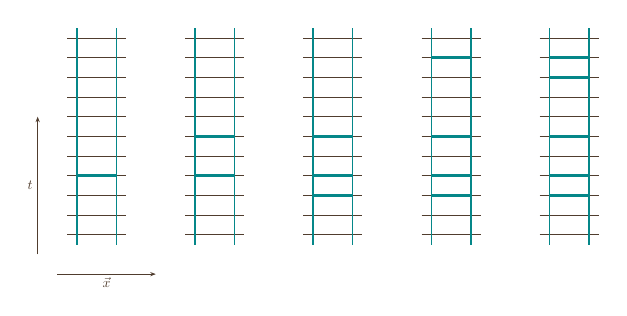
\begin{tikzpicture}
  
  % 1-hop
  % ----------------------------------------------------------------------------
  \begin{scope}[scale=0.5, every node/.style={scale=0.5}]
    % Grid
    % --------------------------------------------------
    \draw[lattice] (-.25,-.25) grid[ystep=0.5,xstep=1] (1.25,5.25);
    %\draw[boundary] (0.1,-.25) -- +(.8,0);
    %\draw[boundary] (0.1,2.75) -- +(.8,0);
    %\draw[boundary] (1.1,-.25) -- +(.8,0);
    %\draw[boundary] (1.1,2.75) -- +(.8,0);
    % --------------------------------------------------
    
    %% Fermion lines
    %% -----------------------------------------------------------
    \begin{scope}
      \clip (-.25,-.25) rectangle (1.25,5.25);
      \draw[link line=ColourHl1] (0,-.25) -- +(0,6);
      \draw[link line=ColourHl1] (1,-.25) -- +(0,6);

      \draw[link line=ColourHl1, line width=1pt] (0,1.5) -- +(1,0);
    \end{scope}
    %% -----------------------------------------------------------
    
  \end{scope}
  % ----------------------------------------------------------------------------

  % 2-hop
  % ----------------------------------------------------------------------------
  \begin{scope}[xshift=1.5cm,scale=0.5, every node/.style={scale=0.5}]
    % Grid
    % --------------------------------------------------
    \draw[lattice] (-.25,-.25) grid[ystep=0.5,xstep=1] (1.25,5.25);
    %\draw[boundary] (0.1,-.25) -- +(.8,0);
    %\draw[boundary] (0.1,2.75) -- +(.8,0);
    %\draw[boundary] (1.1,-.25) -- +(.8,0);
    %\draw[boundary] (1.1,2.75) -- +(.8,0);
    % --------------------------------------------------
    
    %% Fermion lines
    %% -----------------------------------------------------------
    \begin{scope}
      \clip (-.25,-.25) rectangle (1.25,5.25);
      \draw[link line=ColourHl1] (0,-.25) -- +(0,6);
      \draw[link line=ColourHl1] (1,-.25) -- +(0,6);

      \draw[link line=ColourHl1, line width=1pt] (0,1.5) -- +(1,0);
      \draw[link line=ColourHl1, line width=1pt] (0,2.5) -- +(1,0);
    \end{scope}
    %% -----------------------------------------------------------
    
  \end{scope}
  % ----------------------------------------------------------------------------

  % 3-hop
  % ----------------------------------------------------------------------------
  \begin{scope}[xshift=3cm,scale=0.5, every node/.style={scale=0.5}]
    % Grid
    % --------------------------------------------------
    \draw[lattice] (-.25,-.25) grid[ystep=0.5,xstep=1] (1.25,5.25);
    %\draw[boundary] (0.1,-.25) -- +(.8,0);
    %\draw[boundary] (0.1,2.75) -- +(.8,0);
    %\draw[boundary] (1.1,-.25) -- +(.8,0);
    %\draw[boundary] (1.1,2.75) -- +(.8,0);
    % --------------------------------------------------
    
    %% Fermion lines
    %% -----------------------------------------------------------
    \begin{scope}
      \clip (-.25,-.25) rectangle (1.25,5.25);
      \draw[link line=ColourHl1] (0,-.25) -- +(0,6);
      \draw[link line=ColourHl1] (1,-.25) -- +(0,6);

      \draw[link line=ColourHl1, line width=1pt] (0,1.5) -- +(1,0);
      \draw[link line=ColourHl1, line width=1pt] (0,2.5) -- +(1,0);
      \draw[link line=ColourHl1, line width=1pt] (0,1.0) -- +(1,0);
    \end{scope}
    %% -----------------------------------------------------------
    
  \end{scope}
  % ----------------------------------------------------------------------------

  % 4-hop
  % ----------------------------------------------------------------------------
  \begin{scope}[xshift=4.5cm,scale=0.5, every node/.style={scale=0.5}]
    % Grid
    % --------------------------------------------------
    \draw[lattice] (-.25,-.25) grid[ystep=0.5,xstep=1] (1.25,5.25);
    %\draw[boundary] (0.1,-.25) -- +(.8,0);
    %\draw[boundary] (0.1,2.75) -- +(.8,0);
    %\draw[boundary] (1.1,-.25) -- +(.8,0);
    %\draw[boundary] (1.1,2.75) -- +(.8,0);
    % --------------------------------------------------
    
    %% Fermion lines
    %% -----------------------------------------------------------
    \begin{scope}
      \clip (-.25,-.25) rectangle (1.25,5.25);
      \draw[link line=ColourHl1] (0,-.25) -- +(0,6);
      \draw[link line=ColourHl1] (1,-.25) -- +(0,6);

      \draw[link line=ColourHl1, line width=1pt] (0,1.5) -- +(1,0);
      \draw[link line=ColourHl1, line width=1pt] (0,2.5) -- +(1,0);
      \draw[link line=ColourHl1, line width=1pt] (0,1.0) -- +(1,0);
      \draw[link line=ColourHl1, line width=1pt] (0,4.5) -- +(1,0);
    \end{scope}
    %% -----------------------------------------------------------
    
  \end{scope}
  % ----------------------------------------------------------------------------

  % 5-hop
  % ----------------------------------------------------------------------------
  \begin{scope}[xshift=6cm,scale=0.5, every node/.style={scale=0.5}]
    % Grid
    % --------------------------------------------------
    \draw[lattice] (-.25,-.25) grid[ystep=0.5,xstep=1] (1.25,5.25);
    % --------------------------------------------------
    
    %% Fermion lines
    %% -----------------------------------------------------------
    \begin{scope}
      \clip (-.25,-.25) rectangle (1.25,5.25);
      \draw[link line=ColourHl1] (0,-.25) -- +(0,6);
      \draw[link line=ColourHl1] (1,-.25) -- +(0,6);

      \draw[link line=ColourHl1, line width=1pt] (0,1.5) -- +(1,0);
      \draw[link line=ColourHl1, line width=1pt] (0,2.5) -- +(1,0);
      \draw[link line=ColourHl1, line width=1pt] (0,1.0) -- +(1,0);
      \draw[link line=ColourHl1, line width=1pt] (0,4.5) -- +(1,0);
      \draw[link line=ColourHl1, line width=1pt] (0,4.0) -- +(1,0);
    \end{scope}
    %% -----------------------------------------------------------
    
  \end{scope}
  % ----------------------------------------------------------------------------


  %% Axes
  %% --------------------------------------------------------------------------
  \draw[arrows={-Stealth[length=2pt]},thin,ColourDark] (-.25,-.5) -- +(1.25,0) 
    node[midway,below=.4mm,anchor=north,inner sep=0pt, scale=0.5] {$\vec{x}$};
  \draw[arrows={-Stealth[length=2pt]},thin,ColourDark] (-.5,-.25) -- +(0,1.75) 
    node[midway,left=.6mm,anchor=east,inner sep=0pt, scale=0.5] {$t$};
  %% --------------------------------------------------------------------------

\end{tikzpicture}

\end{document}
